\documentclass[12pt]{article}
\usepackage[left=1cm, right=1cm, top=2cm,bottom=1.5cm]{geometry} 

\usepackage[parfill]{parskip}
\usepackage[utf8]{inputenc}
\usepackage[T2A]{fontenc}
\usepackage[russian]{babel}
\usepackage{enumitem}
\usepackage[normalem]{ulem}
\usepackage{amsfonts, amsmath, amsthm, amssymb, mathtools}

\usepackage{tabularx}
\usepackage{hhline}

\usepackage{accents}
\usepackage{fancyhdr}
\pagestyle{fancy}
\renewcommand{\headrulewidth}{1.5pt}
\renewcommand{\footrulewidth}{1pt}

\usepackage{graphicx}
\usepackage[figurename=Рис.]{caption}
\usepackage{subcaption}
\usepackage{float}

%%Наименование папки откуда забирать изображения
\graphicspath{ {./images/} }

%%Изменение формата для ввода доказательства
\renewcommand{\proofname}{$\square$  \nopunct}
\renewcommand\qedsymbol{$\blacksquare$}

%%Изменение отступа на таблицах
\addto\captionsrussian{%
	\renewcommand{\proofname}{$\square$ \nopunct}%
}
%% Римские цифры
\newcommand{\RN}[1]{%
	\textup{\uppercase\expandafter{\romannumeral#1}}%
}

%% Для удобства записи
\newcommand{\MR}{\mathbb{R}}
\newcommand{\MC}{\mathbb{C}}
\newcommand{\MQ}{\mathbb{Q}}
\newcommand{\MN}{\mathbb{N}}
\newcommand{\MZ}{\mathbb{Z}}
\newcommand{\MTB}{\mathbb{T}}
\newcommand{\MTI}{\mathbb{I}}
\newcommand{\MI}{\mathrm{I}}
\newcommand{\MJ}{\mathrm{J}}
\newcommand{\MH}{\mathrm{H}}
\newcommand{\MT}{\mathrm{T}}
\newcommand{\MU}{\mathcal{U}}
\newcommand{\MV}{\mathcal{V}}
\newcommand{\MB}{\mathcal{B}}
\newcommand{\MW}{\mathcal{W}}
\newcommand{\ML}{\mathcal{L}}
\newcommand{\VN}{\varnothing}
\newcommand{\VE}{\varepsilon}

\theoremstyle{definition}
\newtheorem{defn}{Опр:}
\newtheorem{rem}{Rm:}
\newtheorem{prop}{Утв.}
\newtheorem{exrc}{Упр.}
\newtheorem{lemma}{Лемма}
\newtheorem{theorem}{Теорема}
\newtheorem{corollary}{Следствие}

\newenvironment{cusdefn}[1]
{\renewcommand\thedefn{#1}\defn}
{\enddefn}

\DeclareRobustCommand{\divby}{%
	\mathrel{\text{\vbox{\baselineskip.65ex\lineskiplimit0pt\hbox{.}\hbox{.}\hbox{.}}}}%
}
%Короткий минус
\DeclareMathSymbol{\SMN}{\mathbin}{AMSa}{"39}
%Длинная шапка
\newcommand{\overbar}[1]{\mkern 1.5mu\overline{\mkern-1.5mu#1\mkern-1.5mu}\mkern 1.5mu}
%Функция знака
\DeclareMathOperator{\sgn}{sgn}

%Функция ранга
\DeclareMathOperator{\rk}{\text{rk}}

%Обозначение константы
\DeclareMathOperator{\const}{\text{const}}

\DeclareMathOperator*{\dsum}{\displaystyle\sum}
\newcommand{\ddsum}[2]{\displaystyle\sum\limits_{#1}^{#2}}

%Интеграл в большом формате
\DeclareMathOperator{\dint}{\displaystyle\int}
\newcommand{\ddint}[2]{\displaystyle\int\limits_{#1}^{#2}}
\newcommand{\ssum}[1]{\displaystyle \sum\limits_{n=1}^{\infty}{#1}_n}

\newcommand{\smallerrel}[1]{\mathrel{\mathpalette\smallerrelaux{#1}}}
\newcommand{\smallerrelaux}[2]{\raisebox{.1ex}{\scalebox{.75}{$#1#2$}}}

\newcommand{\smallin}{\smallerrel{\in}}
\newcommand{\smallnotin}{\smallerrel{\notin}}

\newcommand*{\medcap}{\mathbin{\scalebox{1.25}{\ensuremath{\cap}}}}%
\newcommand*{\medcup}{\mathbin{\scalebox{1.25}{\ensuremath{\cup}}}}%

\makeatletter
\newcommand{\vast}{\bBigg@{3.5}}
\newcommand{\Vast}{\bBigg@{5}}
\makeatother

%Промежуточное значение для sup\inf, поскольку они имеют разную высоту
\newcommand{\newsup}{\mathop{\smash{\mathrm{sup}}}}
\newcommand{\newinf}{\mathop{\mathrm{inf}\vphantom{\mathrm{sup}}}}

%Скалярное произведение
\DeclarePairedDelimiterX{\inner}[2]{\langle}{\rangle}{#1, #2}

%Подпись символов снизу
\newcommand{\ubar}[1]{\underaccent{\bar}{#1}}

%% Шапка для букв сверху
\newcommand{\wte}[1]{\widetilde{#1}}

%%Функция для обозначения равномерной сходимости по множеству
\newcommand{\uconv}[1]{\overset{#1}{\rightrightarrows}}
\newcommand{\uconvm}[2]{\overset{#1}{\underset{#2}{\rightrightarrows}}}


%%Функция для обозначения нижнего и верхнего интегралов
\def\upint{\mathchoice%
	{\mkern13mu\overline{\vphantom{\intop}\mkern7mu}\mkern-20mu}%
	{\mkern7mu\overline{\vphantom{\intop}\mkern7mu}\mkern-14mu}%
	{\mkern7mu\overline{\vphantom{\intop}\mkern7mu}\mkern-14mu}%
	{\mkern7mu\overline{\vphantom{\intop}\mkern7mu}\mkern-14mu}%
	\int}
\def\lowint{\mkern3mu\underline{\vphantom{\intop}\mkern7mu}\mkern-10mu\int}


\begin{document}
\lhead{Математический анализ - \RN{3}}
\chead{Шапошников С.В.}
\rhead{Лекция - 26}

\section*{Свойства свёртки функций}

\subsection*{Дельтаобразные последовательности}

\begin{defn}
	\uwave{Дельтаобразной последовательностью} функций называется всякая последовательность функций $\{\omega_n\}$, удовлетворяющая свойствам:
	\begin{enumerate}[label=\arabic*)]
		\item $\omega_n$ - интегрируема и $\ddint{-\infty}{+\infty}\omega_n(t)dt = 1$;
		\item $\omega_n \geq 0$;
		\item $\forall \delta > 0, \, \ddint{|t|\geq \delta}{}\omega_n(t)dt \xrightarrow[n \to \infty]{} 0$;
	\end{enumerate}
\end{defn}

Следующая теорема дает представление об искомой единице для свёртки функций.
\begin{theorem}
	Пусть $f$ - непрерывная и ограниченная функция, $\{\omega_n\}$ - это дельтаобразная последовательность. Тогда: $\forall\, [a,b]\subset \MR, \, f *\omega_n(x) \uconvm{[a,b]}{n \to \infty}f(x)$.
\end{theorem} 
\begin{proof}
	Рассмотрим разность между свёрткой и функцией:
	$$
		f*\omega_n(x) - f(x) = \ddint{-\infty}{+\infty}f(t)\omega_n(x-t)dt - f(x) = \ddint{-\infty}{+\infty}f(t)\omega_n(x-t)dt - f(x){\cdot}1 =
	$$
	$$
		= \ddint{-\infty}{+\infty}f(t)\omega_n(x-t)dt - f(x)\,{\cdot}\!\!\ddint{-\infty}{+\infty}\omega_n(t)dt = \ddint{-\infty}{+\infty}f(t)\omega_n(x-t)dt - \ddint{-\infty}{+\infty}f(x)\omega_n(t)dt = 
	$$
	$$
		= \ddint{-\infty}{+\infty}f(x - t)\omega_n(t)dt - \ddint{-\infty}{+\infty}f(x)\omega_n(t)dt = \ddint{-\infty}{+\infty}\left(f(x-t) - f(x)\right)\omega_n(t)dt
	$$
	Хотелось бы понять, бывает ли разность $f(x-t) - f(x)$ маленькой? Да, например, если $t$ - маленькие $\Rightarrow$ надо будет разбить интеграл на два, где $|t| < \delta$ и $|t| \geq \delta$. Тогда на первом интеграле мы воспользуемся свойством непрерывности, а на втором свойством дельтаобразной последовательности. 
	
	По определению, функция $f$ - непрерывна на отрезке $\Rightarrow$ по теореме Кантора равномерно непрерывна на отрезке по $x$, тогда будет верно:
	$$
		\forall \VE > 0, \, \exists \, \delta \in (0,1) \colon \forall x_1, x_2 \in [a-1,b+1], \, |x_1 - x_2| < \delta \Rightarrow |f(x_1) - f(x_2)| < \VE
	$$
	где мы увеличили отрезок с $[a,b]$ до $[a-1,b+1]$, чтобы $x - t$ попадало в этот отрезке:
	$$
		x \in [a,b], \, \delta \in (0,1) \Rightarrow |t| < \delta < 1 \Rightarrow x -t \in [a-1,b+1]
	$$
	Пусть $M = \sup\limits_{\MR}|f|$, он существует по условию ограниченности функции. Оценим разность:
	$$
		\forall x \in [a,b], \, \left|f*\omega_n(x) - f(x)\right|\leq \left|\ddint{-\infty}{\infty} (f(x-t) - f(x))\omega_n(t)dt \right|\leq \ddint{-\infty}{\infty}\left| f(x-t) - f(x)\right|\omega_n(t)dt = 
	$$
	$$
		= \ddint{|t|< \delta}{}\left| f(x-t) - f(x)\right|\omega_n(t)dt + \ddint{|t|\geq \delta}{}\left| f(x-t) - f(x)\right|\omega_n(t)dt \leq \VE{\cdot}1 + 2M \ddint{|t|\geq \delta}{}\omega_n(t)dt
	$$
	По свойству дельтаобразной последовательности: $\exists \, N \colon \forall n > N, \, \ddint{|t|\geq \delta}{}\omega_n(t)dt < \VE$, тогда:
	$$
		\forall x \in [a,b], \, \left|f*\omega_n(x) - f(x)\right|\leq \VE(1 + 2M)
	$$
	И записывая всё вместе, получим равномерную сходимость по определению:
	$$
		\forall \VE > 0, \, \exists \, N \colon \forall n > N, \, \sup\limits_{[a,b]}\left|f*\omega_n(x) - f(x)\right| < \VE
	$$
\end{proof}

\begin{theorem}
	Пусть $f(x)$ и $g(x)$ - непрерывны, хотя бы одна из них финитна и функция $g(x) \in C^k(\MR)$. Тогда: $f*g(x) \in C^k(\MR)$ и будет верно:
	$$
		(f*g)^{(k)}(x) = f*g^{(k)}\,(x)
	$$
\end{theorem}
\begin{rem}
	Заметим, что при поточечном перемножении функций с аналогичными свойстами, если непрерывная функция не является дифференцируемой, то произведение таких функций не будет дифференцируемо, например при $g(x) \equiv 1$, $f(x) \in C(\MR)$ но не дифференцируема $\Rightarrow f(x)g(x) = f(x)$.
\end{rem}
\begin{proof}
	Пусть $x \in (\alpha, \beta)$ - конечный интервал, если функция будет $k$ раз дифференцируема на таком малом интервале, а мы можем взять любой такой интервал, то она будет везде $k$ раз дифференцируема. Поскольку по определению $f(x)$ или $g(x)$ финитны, то: 
	$$
		\exists \, c > 0 \colon \forall x \in (\alpha,\beta), \, \forall |t| \geq c, \, f(t)g(x - t) = 0 \Rightarrow
	$$
	$$
		\Rightarrow f*g(x) = \ddint{-\infty}{+\infty}f(t)g(x-t)dt = \ddint{-c}{c}f(t)g(x - t)dt
	$$
	Таким образом, у нас получился собственный интеграл, где $f$ - непрерывна, $g$ - $k$-раз дифференцируема. По теореме о дифференцировании определенного интеграла мы получим:
	$$
		(f*g)^{(k)}\,(x) = \ddint{-c}{c}f(t)g^{(k)}(x-t)dt = \ddint{-\infty}{+\infty}f(t)g^{(k)}(x-t)dt = f*g^{(k)}\,(x)
	$$
\end{proof}

\newpage
\section*{Примеры применения свёртки}
\subsection*{Фундаментальное решение}
Рассмотрим следующий объект: 
$$
	L y =	y^{(n)} + a_{n-1} y^{(n-1)} + \dotsc + a_0 y, \, \forall k = \overline{0 ,n-1}, \, a_k \in \MR
$$
Пусть $f(x) \in C_0^{\infty}(\MR)$ - бесконечно гладкая финитная функция,  нужно решить уравнение вида: 
$$
	Ly =f
$$ 
Обычно решается через решение однородного уравнения, а затем решение частного производится через систему уравнений. Но можно решение и угадать.
\begin{prop}
	Пусть $u$ - решение следующей задачи Коши:
	$$
		\left\{
		\begin{array}{rcl}
			Lu &=& 0\\
			u(0) &=& u'(0) = \dotsc = u^{(n-2)}(0) = 0\\
			u^{(n-1)}(0) &=& 1
		\end{array}
		\right.
	$$
	Одновременно с этим, определим функцию: 
	$$
		E(x) = \left\{
		\begin{array}{rl}
			u(x), & x \geq 0\\
			0, & x < 0
		\end{array}
		\right.
	$$
	Тогда: $y(x) = E*f(x)$ - решение $Ly =f$, где $E(x)$ принято называть \uwave{фундаментальным решением}.
\end{prop}
\begin{rem}
	Заметим, что это задача - частный случай мотивационного примера про прибор, где мы подаем сигнал в виде $f(x)$ и получаем отклик в виде $Ly$. Этот прибор обладает свойством линейности и перестановочности со сдвигом по времени. Тогда мы знаем, что работа прибора должна описываться всего лишь одной аппаратной функцией.
\end{rem}
\begin{proof}
	Поскольку $f$ - финитная и бесконечно гладкая функция, $E(x)$ - $(n-2)$-раза дифференцируемая функция (по условию для точки $0$), то мы можем применить предыдущую теорему:
	$$
		y^{(k)}(x) = E*f^{(k)}(x) = \ddint{-\infty}{+\infty}E(t)f^{(k)}(x-t)dt = \ddint{0}{+\infty}u(t)f^{(k)}(x-t)dt
	$$
	Поскольку мы знаем как устроены производные функции $u(t)$, то было бы удобно перебросить производную $(k)$-го порядка на $u(t)$, тогда:
	$$
		f^{(k)}(x-t) = \dfrac{d^k}{dt^k}\left((-1)^kf(x-t)\right) \Rightarrow \ddint{0}{+\infty}u(t)f^{(k)}(x-t)dt = \ddint{0}{+\infty}u(t){\cdot}\dfrac{d^k}{dt^k}\left((-1)^kf(x-t)\right)dt =
	$$
	$$
		= u(t){\cdot}\dfrac{d^{k-1}}{dt^{k-1}}\left((-1)^kf(x-t)\right)\Big|_{t= 0}^{+\infty} - \ddint{0}{+\infty}u'(t){\cdot}\dfrac{d^{k-1}}{dt^{k-1}}\left((-1)^kf(x-t)\right)dt = 
	$$
	$$	
		= - 0{\cdot}\dfrac{d^{k-1}}{dt^{k-1}}\left((-1)^kf(x)\right) + \lim\limits_{b\to \infty}u(b)\dfrac{d^{k-1}}{dt^{k-1}}\left((-1)^kf(x-b)\right) -
	$$
	$$
		- \ddint{0}{+\infty}u'(t){\cdot}\dfrac{d^{k-1}}{dt^{k-1}}\left((-1)^kf(x-t)\right)dt =	- \ddint{0}{+\infty}u'(t){\cdot}\dfrac{d^{k-1}}{dt^{k-1}}\left((-1)^kf(x-t)\right)dt
	$$
	где мы сначала воспользовались интегрированием по частям, а затем значением функции $u(t)$ в нуле (через задачу Коши) и финитностью функции $f(x)$. Продолжим пользоваться формулой интегрирования по частям далее:
	$$
		-\ddint{0}{+\infty}u'(t){\cdot}\dfrac{d^{k-1}}{dt^{k-1}}\left((-1)^kf(x-t)\right)dt =  -u'(t){\cdot}\dfrac{d^{k-2}}{dt^{k-2}}\left((-1)^kf(x-t)\right)\Big|_{t= 0}^{+\infty} +
	$$
	$$
		+ \ddint{0}{+\infty}u''(t){\cdot}\dfrac{d^{k-2}}{dt^{k-2}}\left((-1)^kf(x-t)\right)dt = \ddint{0}{+\infty}u''(t){\cdot}\dfrac{d^{k-2}}{dt^{k-2}}\left((-1)^kf(x-t)\right)dt = \dotsc
	$$
	Рассмотрим случай $k \leq n-1$, тогда получим:
	$$
		y^{(k)}(x) = (-1)^{2k}\ddint{0}{+\infty}u^{(k)}f(x-t)dt = \ddint{0}{+\infty}u^{(k)}f(x-t)dt
	$$
	При $k = n$, в результате ситуация немного изменится:
	$$
		y^{(n)}(x) = (-1)^{n-1}u^{(n-1)}(t){\cdot}\left((-1)^nf(x-t)\right)\Big|_{t= 0}^{+\infty} + (-1)^n\ddint{0}{+\infty}u^{(n)}(t)(-1)^nf(x-t)dt =
	$$
	$$
		=\lim\limits_{b \to \infty}(-1)^{2n -1}u^{(n-1)}(b)f(x-b) - (-1)^{2n-1}u^{(n-1)}(0)f(x) + (-1)^{2n}\ddint{0}{+\infty}u^{(n)}(t)f(x-t)dt =
	$$
	$$
		= f(x) + \ddint{0}{+\infty}u^{(n)}(t)f(x-t)dt
	$$
	Подставим полученые формулы в $Ly(x)$, внесем всё под один интеграл и получим:
	$$
		Ly(x) = y^{(n)}(x) + a_{n-1} y^{(n-1)}(x) + \dotsc + a_0 y(x) = f(x) +
	$$
	$$
		+  \ddint{0}{+\infty}\left(u^{(n)}(t) + a_{n-1}u^{(n-1)}(t) + \dotsc + a_0 u(t)\right){\cdot}f(x-t)dt = f(x) + \ddint{0}{+\infty}0{\cdot}f(x-t)dt = f(x)
	$$
\end{proof}

\textbf{Пример}: Решить уравнение: $y'' + y = f$ с задачей Коши: $\left\{
\begin{array}{rcl}
	u''(t) + u(t) &=& 0\\
	u(0) &=& 0, \, u'(0) = 1
\end{array}
\right.
$.
\begin{proof}
	Из задачи Коши сразу следует, что $u(t) = \sin{t}$, тогда $y(x) = \ddint{0}{+\infty}\sin{t}{\cdot}f(x - t)dt$.
\end{proof}
\begin{rem}
	Заметим, что эта формула работает не только для финитных носителей.
\end{rem}
\newpage
\subsection*{Теорема Вейерштрасса}
\begin{theorem}(\textbf{Вейерштрасс})
	Если $f \in C([a,b])$, то $\exists\, P_n$ - многочлены: $P_n \uconvm{[a,b]}{n \to \infty}f$.
\end{theorem}
\begin{proof}
	Доопределим функцию $f(x)$ так, чтобы она была непрерывной и финитной на $\MR$. Тогда найдется такое $c > 0$, что $f(x) \equiv 0, \, \forall x \in \MR\ \setminus [-c,c]$.
	\begin{figure}[H]
		\centering
		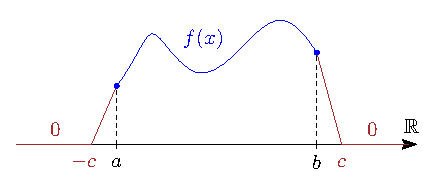
\includegraphics[width=0.45\textwidth]{MA3L26_1.eps}
		\label{MA3L26_1}
		\caption{Доопределение функции $f(x)$ до непрерывной и финитной на $\MR$.}
		\label{fig: Доопределение функции}
	\end{figure}
	В качестве $\delta$-образной последовательности возьмем: $\omega_n(x) = n\psi(nx)$, где $\psi(x) = \tfrac{1}{\sqrt{2\pi}}e^{-\tfrac{x^2}{2}}$. По сути это плотность нормального распределения (см. лекцию $8$):
	$$
		\ddint{-\infty}{+\infty}\psi(x)dx = \ddint{-\infty}{+\infty}\dfrac{1}{\sqrt{2\pi}}e^{-\tfrac{x^2}{2}} dx = 1, \, \psi(x) \geq 0, \, \forall x \in \MR
	$$
	также заметим, что $\omega_n(x)$ - бесконечно гладкая функция $\Rightarrow f*\omega_n(x)$ - тоже бесконечно гладкая $\Rightarrow$ её легче приближать многочленом, чем просто непрерывную функцию. По теореме $1$ мы знаем, что свёртка будет равномерно сходиться: 
	$$
		f*\omega_n(x) \uconvm{[a,b]}{n \to \infty}f(x)
	$$ 
	Следовательно, достаточно приблизить многочленами функцию $f * \omega_n(x)$ при фиксированном $n$: приблизили $f*\omega_n(x)$ многочленом с зазором $\VE$, а $f*\omega_n(x)$ приблизили к $f(x)$, также с зазором $\VE$, тогда мы приблизили $f(x)$ многочленом с зазором в $2\VE$. Фиксируем $n$, тогда:
	$$
		f*\omega_n(x) = \ddint{-\infty}{+\infty}f(t)\dfrac{n}{\sqrt{2 \pi}}e^{-\tfrac{n^2(x-t)^2}{2}}dt = \dfrac{n}{\sqrt{2 \pi}}\ddint{-c}{c}f(t)e^{-\tfrac{n^2(x-t)^2}{2}}dt
	$$
	Чтобы появились многочлены по переменной $x$ необходимо разложить экспоненту в ряд Тейлора. Поскольку $x \in [a,b], \, t \in [-c,c]$, то:
	$$
		\forall x \in [a,b], \, \forall  t \in [-c,c], \, \exists \, M > 0\colon n^2(x - t)^2 \leq M \Rightarrow
	$$
	$$
		\Rightarrow \forall x \in [a,b], \, \forall  t \in [-c,c], \, e^{-\tfrac{n^2(x-t)^2}{2}} = \ddsum{k = 0}{\infty}\dfrac{(-1)^k n^{2k}(x-t)^{2k}}{2^k k!} \Rightarrow \ddsum{k = K}{\infty} \left|\dfrac{(-1)^k n^{2k}(x-t)^{2k}}{2^k k!}\right| \leq \ddsum{k = K}{\infty}\dfrac{M^k}{k!} \to 0
	$$
	Таким образом, мы получаем равномерную сходимость ряда при указанных $x$ и $t \Rightarrow$ можно переставить ряд с интегралом, тогда: 
	$$
		f*\omega_n(x) = \dfrac{n}{\sqrt{2 \pi}}\ddint{-c}{c}f(t)e^{-\tfrac{n^2(x-t)^2)}{2}}dt = \dfrac{n}{\sqrt{2 \pi}}\ddsum{k = 0}{\infty}\dfrac{(-1)^k n^{2k}}{2^k k!}\ddint{-c}{c}f(t)(x-t)^{2k}dt
	$$
	Рассмотрим хвост получившегося ряда:
	$$
		\ddsum{k = K}{\infty}\left|\dfrac{(-1)^k n^{2k}}{2^k k!}\ddint{-c}{c}f(t)(x-t)^{2k}dt\right| = \ddsum{k = K}{\infty}\left|\dfrac{(-1)^k}{2^k k!}\ddint{-c}{c}f(t)n^{2k}(x-t)^{2k}dt\right| 
		\leq \ddsum{k = K}{\infty}\dfrac{M^{k}\int\limits_{-c}^{c}|f(t)|dt}{k!}
	$$	
	где интеграл в числителе это всего лишь константа. Как мы можем видеть, получившаяся оценка не зависит от $x \Rightarrow$ ряд сходится равномерно к $f*\omega_n(x)$ на $[a,b]$. Осталось заметить, что выражения вида:
	$$
		\ddint{-c}{c}f(t)(x-t)^{2k}dt = \ddint{-c}{c}f(t)\ddsum{j = 0}{2k}C_{2k}^{j}x^j(-1)^{2k-j}t^{2k-j}dt = \ddsum{j = 0}{2k}C_{2k}^{j}x^j(-1)^{2k-j}\ddint{-c}{c}f(t)t^{2k-j}dt
	$$
	есть ничто иное, как многочлен по $x$
\end{proof}
\begin{rem}
	Доказывая теорему Вейерштрасса, мы параллельно доказали, что мы можем непрерывную функцию приблизить гладкой. Свёртка хороша тем, что она это делает явно.
\end{rem}

\newpage
\section*{Свёртка периодических функций}
На практике бывает полезно использовать свёртку для периодических функций. Пусть $f$ и $g$ - интегрируемы на отрезке $[0,T]$ и $T$-периодические: $\forall x \in \MR, \, f(x + T) = f(x), \, g(x + T) = g(x)$.
\begin{defn}
	\uwave{Свёртка периодических функций} определяется следующим образом:
	$$
		f*g(x) = \ddint{0}{T}f(t)g(x - t)dt, \, \forall x \in \MR
	$$
\end{defn}
Заметим, что эта свёртка обладает всеми теми же свойствами, что и обычная на $\MR$. Далее мы проверим те из них, которые нам понадобятся в дальнейшем.
\begin{rem}
	Сразу отметим, что никаких условий существования интеграла свёртки не нужно, поскольку достаточно интегрируемости функций $f$ и $g$: в определенном интеграле произведение двух интегрируемых функций это интегрируемая функция.
\end{rem}

\begin{lemma}
	Если $f$ - $T$-периодическая и интегрируемая по Риману, то верно:
	$$
		\forall a \in \MR, \, \ddint{a}{a +T}f(t)dt = \ddint{0}{T}f(t)dt
	$$
\end{lemma}
\begin{proof}
	Сдвигая на $kT$, можно считать, что $0 \leq a < T$.
	\begin{figure}[H]
		\centering
		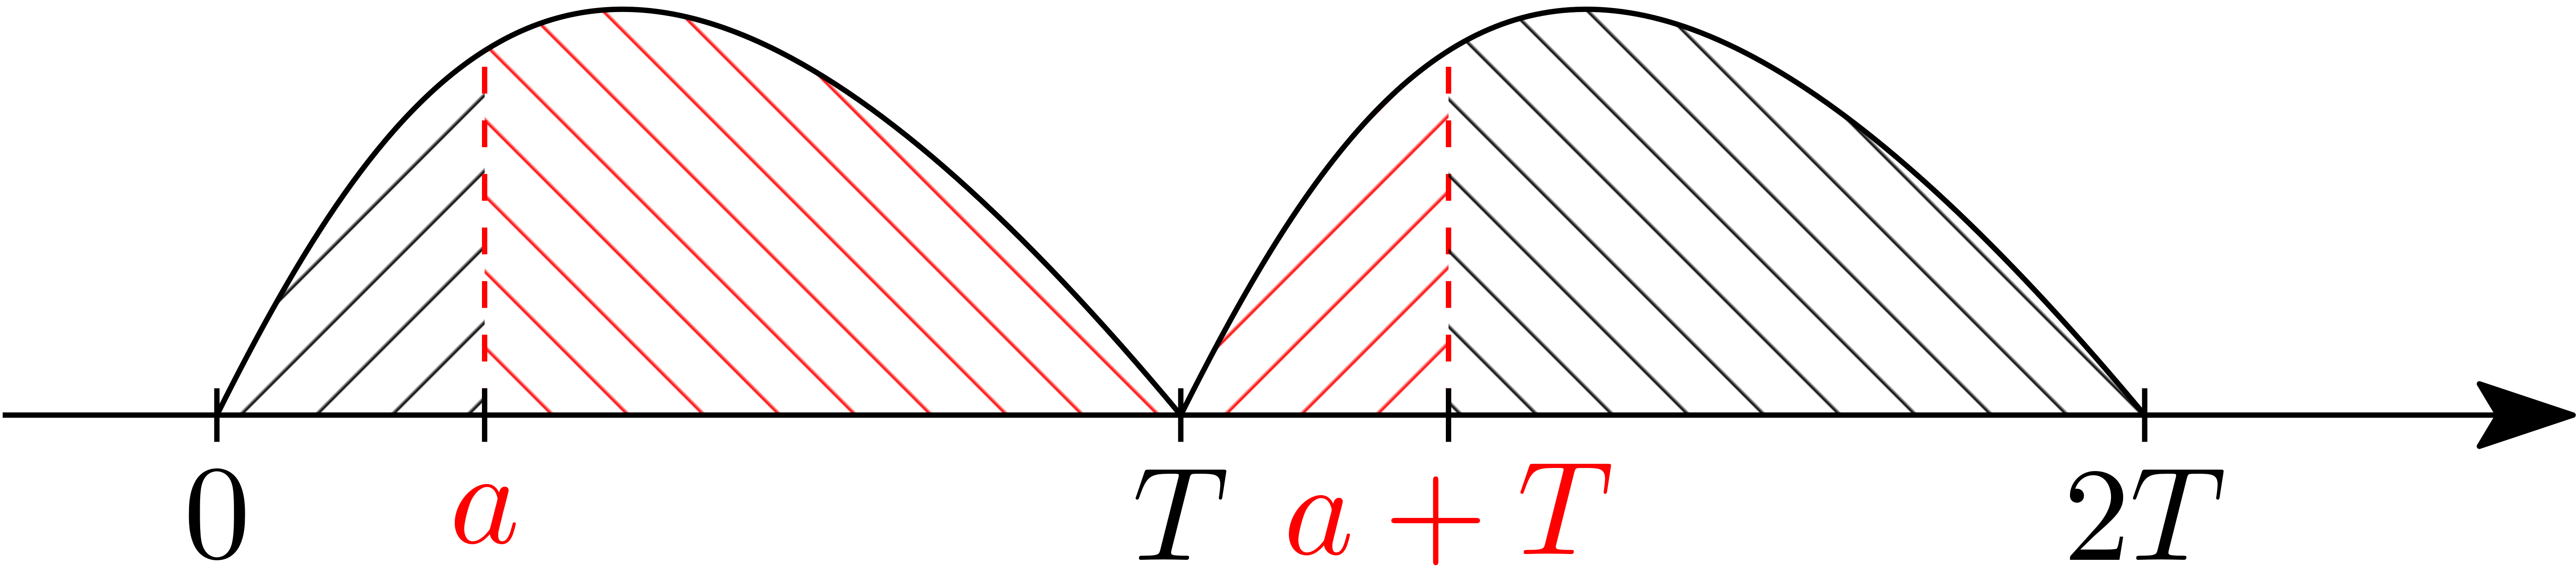
\includegraphics[width=0.65\textwidth]{MA3L26_2.png}
		\label{MA3L26_2}
		\caption{Сдвиг промежутка интегрирования на $a \in \MR$ для периодической функции.}
		\label{fig: Сдвиг промежутка интегрирования}
	\end{figure}
	Воспользуемся периодичностью функции и сделаем замену переменной под интегралом:
	$$
		\ddint{0}{a}f(t)dt = \ddint{0}{a}f(t + T)dt = \ddint{T}{a + T}f(t)dt \Rightarrow \ddint{0}{T}f(t)dt  = \ddint{0}{a}f(t)dt + \ddint{a}{T}f(t)dt = 
	$$
	$$
		= \ddint{T}{a + T}f(t)dt + \ddint{a}{T}f(t)dt =  \ddint{a}{T}f(t)dt + \ddint{T}{a + T}f(t)dt  = \ddint{a}{a + T}f(t)dt
	$$
\end{proof}
\begin{exrc}
	Пусть $f$ - непрерывная функция такая, что:
	$$
		\forall a \in \MR, \, \ddint{a}{a+T}f(t)dt = \ddint{0}{T}f(t)dt
	$$
	Верно ли, что $f$ - $T$-периодическая?
\end{exrc}
\begin{proof}
	Сдвигая на $kT$, можно считать, что $0 \leq a < T$. Рассмотрим свойство функции:
	$$
		\ddint{a}{a + T}f(t)dt = \ddint{a}{T}f(t)dt + \ddint{T}{a + T}f(t)dt = \ddint{0}{T}f(t)dt \Rightarrow \ddint{T}{a +T}f(t)dt = \ddint{0}{T}f(t)dt + \ddint{T}{a}f(t)dt \Rightarrow
	$$
	$$
		\Rightarrow \ddint{T}{a + T}f(t)dt = |t = s +T| = \ddint{0}{a}f(s + T)ds = \ddint{0}{a}f(t)dt
	$$
	Поскольку $f$ - непрерывная, то продифференцируем интегралы по параметру $a$:
	$$
		\dfrac{d}{da}\left(\ddint{0}{a}f(s + T)ds\right) = 1{\cdot}f(a + T) = f(a + T) = \dfrac{d}{da}\left(\ddint{0}{a}f(t)dt\right) = f(a) , \, \forall a \in \MR
	$$
\end{proof}

\begin{theorem} Выполнены следующие свойства:
	\begin{enumerate}[label=\arabic*)]
		\item $f*g(x)$ - $T$-периодическая функция;
		\item $f*g(x) = g*f(x)$;
		\item Если $f(x)$ - непрерывна, а $g(x) \in C^k(\MR)$, то $f*g(x) \in C^k(\MR)$ и $(f*g)^{(k)}(x) = f*g^{(k)}(x)$;
	\end{enumerate}
\end{theorem}
\begin{proof}
	По определению: $f*g(x) = \ddint{0}{T}f(t)g(x - t)dt$, тогда:
	\begin{enumerate}[label=\arabic*)]
		\item $f*g(x + T) = \ddint{0}{T}f(t)g(x - t + T)dt = \ddint{0}{T}f(t)g(x - t )dt = f*g(x)$, так как $g(x)$ - $T$-периодическая;
		\setcounter{enumi}{2}
		\item Используя дифференцирование по параметру собственного интеграла получаем требуемое;
		\setcounter{enumi}{1}
		\item Поскольку $f$ и $g$ это $T$-периодические функции, то $f{\cdot}g$ - тоже $T$-периодическая. Проверим свойство:
		$$
			f*g(x) = \ddint{0}{T}f(t)g(x-t)dt = |x -t = s| =  \ddint{x- T}{x}f(x-s)g(s)ds = \ddint{0}{T}f(x-s)g(s)ds = g*f(x)
		$$
		где в предпоследнем равенстве мы воспользовались леммой $1$ при $x - T = a$ и $x = a + T$;
	\end{enumerate}
\end{proof}

\newpage
\subsection*{Дельтаобразная последовательность $T$-периодических функций}
Аналогично свёртке на всей прямой для свёртки $T$-периодических функций возникает проблема с единицей и мы вновь вводим определение дельтаобразной последовательности.
\begin{defn}
	Последовательность интегриуремых $T$-периодических функций $\omega_n$ называется \uwave{дельтаобразной последовательностью}, если выполнены следующие свойства:
	\begin{enumerate}[label=\arabic*)]
		\item $\forall x \in \MR, \, \omega_n(x) \geq 0$;
		\item $\ddint{0}{T}\omega_n(t)dt = 1$;
		\item $\forall \delta \in (0,T), \, \ddint{\delta}{T - \delta}\omega_n(t)dt \xrightarrow[n \to \infty]{} 0$;
	\end{enumerate}
\end{defn}

\textbf{Пример}: Пусть $\omega_n(t) = c_n{\cdot}\cos^{2n}{\tfrac{t}{2}}$, где $c_n = \dfrac{1}{\int\limits_{0}^{2\pi}\cos^{2n}{\tfrac{t}{2}}dt}$ и $T = 2\pi$. Проверим, что это $\delta$-образная последовательность. 
\begin{proof}\hfill
	\begin{enumerate}[label=\arabic*)]
		\item $\forall t \in \MR, \, \forall n \in \MN, \, \cos^{2n}{\tfrac{t}{2}} \geq 0 \Rightarrow c_n \geq 0 \Rightarrow \omega_n(t) \geq 0$;
		\item $\ddint{0}{2\pi}\omega_n(t)dt = c_n\ddint{0}{2\pi}\cos^{2n}{\tfrac{t}{2}}dt = \dfrac{\int\limits_{0}^{2\pi}\cos^{2n}{\tfrac{t}{2}}dt}{\int\limits_{0}^{2\pi}\cos^{2n}{\tfrac{t}{2}}dt} = 1$;
		\item Пусть $\delta \in (0, 2\pi)$, тогда: 
		$$
			\forall \tfrac{t}{2} \in \left(\tfrac{\delta}{2}, \pi - \tfrac{\delta}{2}\right) \Rightarrow \cos^{2n}{\tfrac{t}{2}} \leq \cos^{2n}{\tfrac{\delta}{2}} \xrightarrow[n\to\infty]{} 0
		$$ 
		где последнее верно, так как $\cos^{2n}{\tfrac{\delta}{2}} < 1$. Хотелось бы понять, как себя ведёт $c_n$, поскольку там идёт деление на интеграл, то нужно оценивать его снизу:
		$$
			\ddint{0}{2\pi}\cos^{2n}{\tfrac{t}{2}}dt = 2\ddint{0}{\pi}\cos^{2n}tdt = 2\ddint{-\frac{\pi}{2}}{\frac{\pi}{2}}\cos^{2n}tdt = 4 \ddint{0}{\frac{\pi}{2}}\cos^{2n}tdt
		$$
		где в последнем равенстве мы воспользовались чётностью подинтегральной функции. Сделаем замену: $\cos{t} = z \Rightarrow dz = -\sin{t}dt = -\sqrt{1- z^2}dt$, тогда:
		$$
			4 \ddint{0}{\frac{\pi}{2}}\cos^{2n}tdt = 4 \ddint{0}{1}\dfrac{z^{2n}}{\sqrt{1 - z^2}}dz = |z^2 = u \Rightarrow 2zdz = 2u^{\frac{1}{2}}dz = du| = 2\ddint{0}{1}u^{n -\frac{1}{2}}(1-u)^{-\frac{1}{2}}du = 
		$$
		$$
			= 2\MB\left(n + \tfrac{1}{2}, \tfrac{1}{2}\right) = 2\dfrac{\Gamma\left(n + \frac{1}{2}\right)\Gamma\left(\frac{1}{2}\right)}{\Gamma(n+1)} = 2\Gamma\left(\tfrac{1}{2}\right)\dfrac{\left(n - \frac{1}{2}\right)\Gamma\left(n - \frac{1}{2}\right)}{n\Gamma(n)} = \dotsc =
		$$
		$$
			= 2\Gamma\left(\tfrac{1}{2}\right)\dfrac{\left(n - \frac{1}{2}\right){\cdot}\left(n - 1- \frac{1}{2}\right){\cdot}\dotsc{\cdot}\tfrac{3}{2}{\cdot}\tfrac{1}{2}{\cdot}\Gamma\left(\tfrac{1}{2}\right)}{n{\cdot}(n-1){\cdot}(n-2){\cdot}\dotsc{\cdot}1} \geq 2 \pi{\cdot}\dfrac{1}{2n} = \dfrac{\pi}{n}
		$$
		Следовательно, мы можем оценить следующее слагаемое:
		$$
			\dfrac{\int\limits_{\delta}^{2\pi - \delta}\cos^{2n}{\tfrac{t}{2}}dt}{\int\limits_{0}^{2\pi}\cos^{2n}{\tfrac{t}{2}}dt} \leq \dfrac{2\pi \cos^{2n}{\tfrac{\delta}{2}}}{\tfrac{\pi}{n}} = 2n\cos^{2n}{\tfrac{\delta}{2}} = 2n a^{2n}, \, a = \cos{\tfrac{\delta}{2}} < 1 \Rightarrow  2n a^{2n} \xrightarrow[n \to \infty]{} 0
		$$
	\end{enumerate}
\end{proof}
\begin{rem}
	Заметим, что в пункте $3)$ оценку снизу можно было дать гораздо проще. Воспользуемся формулой приведения: $\sin{\left(\frac{\pi}{2} + t\right)} = \cos{t}$, тогда:
	$$
		\ddint{0}{2\pi}\cos^{2n}{\tfrac{t}{2}}dt = 2\ddint{0}{\pi}\cos^{2n}tdt = 2\ddint{0}{\pi}\sin^{2n}{\left(t + \tfrac{\pi}{2}\right)}dt = 2 \ddint{-\tfrac{\pi}{2}}{\tfrac{\pi}{2}}\sin^{2n}{t}dt = 4\ddint{0}{\tfrac{\pi}{2}}\sin^{2n}{t}dt
	$$
	где мы опять воспользовались четностью подинтегральной функции, используя неравенство: 
	$$
		\sin{x} \geq \dfrac{2x}{\pi}, \, \forall x \in \left[0,\dfrac{\pi}{2}\right]
	$$ 
	мы получим оценку снизу:
	$$
		4\ddint{0}{\tfrac{\pi}{2}}\sin^{2n}{t}dt \geq 4\ddint{0}{\tfrac{\pi}{2}}\left(\dfrac{2t}{\pi}\right)^{2n}dt = 2\pi\ddint{0}{1}s^{2n}ds = \dfrac{2\pi}{2n + 1}
	$$
\end{rem}

\begin{theorem}
	Пусть $f$ - непрерывная $T$-периодическая функция и $\{\omega_n\}$ - дельтаобразная последовательность. Тогда на всей прямой (или что тоже самое на $[0,T]$) будет верно: $f*\omega_n(x) \uconvm{[0,T]}{n \to \infty}f$.
\end{theorem}
\begin{proof}
	Аналогично теореме для обычной свёртки, рассмотрим разность $f*\omega_n(x)-f(x)$ и оценим её:
	$$
		f*\omega_n(x) - f(x) = \ddint{0}{T}(f(x-t)-f(x))\omega_n(t)dt \Rightarrow |f*\omega_n(x) - f(x)| \leq \ddint{0}{T}|f(x-t) - f(x)|\omega_n(t)dt 
	$$
	Поскольку функция $f$ - непрерывная и $T$-периодическая, то она равномерно непрерывна на отрезке (по теореме Кантора) $\Rightarrow$ равномерно непрерывна всюду на числовой прямой:
	$$
		\forall \VE > 0, \, \exists \, \delta > 0 \colon \forall x_1, x_2, \, |x_1 - x_2| < \delta \Rightarrow |f(x_1) - f(x_2)| < \VE
	$$
	Из периодичности и непрерывности функции $f$ также следует существование $M = \max\limits_{[0,T]}f = \max\limits_{\MR}f$. Тогда оценим интересующий нас интеграл:
	$$
		\ddint{0}{T}|f(x-t) - f(x)|\omega_n(t)dt = \ddint{0}{\delta}|f(x-t) - f(x)|\omega_n(t)dt + \ddint{T-\delta}{T}|f(x-t) - f(x)|\omega_n(t)dt +
	$$
	$$
		+ \ddint{\delta}{T - \delta}|f(x-t) - f(x)|\omega_n(t)dt = \ddint{0}{\delta}|f(x-t) - f(x)|\omega_n(t)dt + \ddint{-\delta}{0}|f(x-t) - f(x)|\omega_n(t)dt + 
	$$
	$$
		+ \ddint{\delta}{T - \delta}|f(x-t) - f(x)|\omega_n(t)dt = \ddint{|t|<\delta}{}|f(x-t) - f(x)|\omega_n(t)dt + \ddint{\delta}{T - \delta}|f(x-t) - f(x)|\omega_n(t)dt \leq
	$$
	$$
		\leq \VE\ddint{|t|<\delta}{}\omega_n(t)dt + 2M\ddint{\delta}{T - \delta}\omega_n(t)dt \leq \VE + 2M\ddint{\delta}{T - \delta}\omega_n(t)dt
	$$
	По определению дельтаобразной последовательности:
	$$
		\exists \, N \colon \forall n > N, \, \ddint{\delta}{T- \delta}\omega_n(t)dt < \VE 
	$$
	Следовательно, мы получаем требуемое:
	$$
		\forall \VE > 0, \, \exists \, N \colon \forall n > N, \, |f*\omega_n(x) - f(x)| \leq \VE + 2M\ddint{\delta}{T - \delta}\omega_n(t)dt < 2\VE
	$$
\end{proof}

\newpage
\subsection*{Теорема Вейерштрасса}
\begin{defn}
	Выражение вида: 
	$$
		T_n(t) = \dfrac{a_0}{2} + \ddsum{k = 1}{n}(a_k\cos{kt} + b_k\sin{kt})
	$$ 
	называется \uwave{тригонометрическим многочленом}.
\end{defn}
\begin{rem}
	Заметим, что тригонометрический многочлен это просто линейная комбинация тригонометрических функций и единицы: $1, \, \sin{kt},\, \cos{kt}$.
\end{rem}
\begin{exrc}
	Полезно иметь в виду, что сумма и произведение тригонометрических многочленов это тригонометрический многочлен.
\end{exrc}
\begin{theorem}(\textbf{Вейерштрасса})
	Если $f$ - $2\pi$-периодическая и непрерывная функция, то $\exists$ последовательность тригонометрических многочленов $T_N$ такая, что: $T_N \uconvm{\MR}{N \to \infty} f$.	
\end{theorem}
\begin{rem}
	Эту теорему можно получить как следствие теоремы Вейерштрасса для обычной свёртки.
\end{rem}
\begin{proof}
	Возьмем $\omega_n(t) = c_n\cos^{2n}{\frac{t}{2}}$, а в качестве многочлена возьмем свёртку: $T_n(x) = f*\omega_n(x)$. Из предыдущей теоремы мы знаем, что: 
	$$
		T_n(x) \uconvm{\MR}{n\to \infty}f(x)
	$$ 
	Рассмотрим функцию $T_n(x)$ по определению:
	$$
		T_n(x) = c_n \ddint{0}{2\pi}f(t)\cos^{2n}{\left(\tfrac{x-t}{2}\right)}dt = c_n \ddint{0}{2\pi}f(t)\left(\dfrac{\cos{(x-t)} + 1}{2}\right)^n dt =
	$$
	$$
		= \dfrac{c_n}{2^n}\ddint{0}{2\pi}f(t)(\cos{x}\cos{t} + \sin{x}\sin{t} + 1)^n dt
	$$
	Отсюда уже видно, что при раскрытии степеней мы получим тригонометрический многочлен.
\end{proof}

\end{document}